\documentclass[a4paper, 12pt]{article}
\usepackage[french]{babel}
\usepackage[T1]{fontenc}
\usepackage[utf8]{inputenc}
\usepackage[left=2cm,right=2cm,top=3cm,bottom=2cm]{geometry}
\usepackage{graphicx}
\usepackage{xcolor}
\usepackage{color}
\usepackage{ulem}
\usepackage{setspace}
\usepackage{fancyhdr}
\usepackage{float} 
\usepackage[section,above,below]{placeins}
\usepackage[final]{pdfpages}
\usepackage[backend=bibtex]{biblatex}
\bibliography{bibliographie.bib}

\renewcommand{\contentsname}{Sommaire}

\usepackage{footnote}

\begin{document}

\begin{titlepage}
	\centering
	
\includegraphics[width=1\textwidth]{univ.jpg}\par\vspace{1cm}
	{\scshape\LARGE  Projet de Programmation \par}
	\vspace{1cm}
	{\scshape\Large\bfseries Le Clicodrome pour Lexique Electronique \par}
	\vspace{1.5cm}
	{\huge\bfseries MEMOIRE \par}
	\vspace{1.5cm}
	
	
	{\Large\itshape\bfseries ROUSSEL Damien \par}
	\vspace{0.2cm}
	{\Large\itshape\bfseries DIALLO Abdoul  \par}	
	\vspace{0.2cm}
	{\Large\itshape\bfseries EL GUERCH Souhail\par}
	\vspace{0.2cm}
	{\Large\itshape\bfseries MEHDAOUI Abdelamine \par}
	\vspace{0.2cm}
	{\Large\itshape\bfseries DAOUDI Yassir\par}

	\vspace{5cm}
	
	
	{\Large\bfseries Master 1 Informatique   \par}
	\vspace{0.5cm}
	{\Large\bfseries Année universitaire: 2019/2020   \par}
	
	
% Bottom of the page
	\vspace{0.5cm}
	{\large\bfseries \today\par}
\end{titlepage}

\tableofcontents
\newpage
\listoffigures
\newpage

\section{Introduction}
\subsection{Contexte}
Dans le cadre de notre Cursus de Master 1 Informatique à l'Université de bordeaux, nous devons au compte de l'unité d'enseignement Projet de Programmation réalisé par groupe de cinq étudiants un projet de développement informatique. Nous travaillons avec Monsieur \textbf{Lionel CLEMENT} notre client et monsieur \textbf{Simon ARCHIPOFF} chargé de l'encadrement de nos travaux dirigés.


{\textbf{Lionel CLEMENT}, spécialisé dans le domaine de la linguistique formelle et du traitement automatique des langues est un enseignant chercheur au Laboratoire Bordelais de Recherche en Informatique(\textbf{LABRI}). Il a réalisé avec \textbf{Benoit SAGOT} \cite{lefff_int} chercheur à l'Institut National de Recherche en Informatique et Automatique(\textbf{INRIA})  le Lexique électronique des formes fléchies du français, qu'ils ont appelé \textbf{LeFFF}\cite{tagset}\cite{lefff}.\par}
{Le français est une langue, une langue peut-être définie comme un ensemble de signes oraux et écrits qui permettent à un groupe d'individus de communiquer. Les mots qui forment le français se repartissent en neuf classes: les noms, les déterminants, les adjectifs qualificatifs, les pronoms, les verbes, les adverbes,les prépositions, les conjonctions de coordination et les interjections. Partant de cette classification on peut dire que les formes fléchies d'un mot correspondent aux différentes déclinaisons de ce mot (sa conjugaison pour un verbe, son singulier et son pluriels pour certaines catégories de mots, ses synonymes,...etc...).\par}
{Dans le \textbf{LAROUSSE}, un \textit{\bf lexique} est un dictionnaire spécialisé et généralement succinct concernant un domaine particulier de la connaissance, c'est une ressource complexe constituée de \textit{lexèmes}, de \textit{vocables}, de \textit{catégories} et \textit{sous-catégories syntaxiques}, de \textit{catégories grammaticales}, de \textit{règles de flexion}, de \textit{valence}, de \textit{phraséologie}, de \textit{fonctions lexicales},...etc... .\par}

{Habituellement un dictionnaire est utilisé pour trouver la signification d'un mot qu'on connaît et il n'offre pas la possibilité de faire l'inverse, c'est à dire qu'à partir d'explications ou d'une liste de mots trouver le mot correspondant (un gain de temps considérable pour tous).\par}

{L'objectif de ce projet est donc d'implémenter une application Web liée à une base de données(qui contiendra les mots du lexique) pour faciliter les interactions avec le lexique (consultation, ajout, suppression,...).\par}


\subsection{Analyse de l'existant}

\subsubsection{Le lexique: leFFF}
{Le \textbf{LeFFF} est un fichier texte contenant une base de mots, mais il n'existe aucun outil qui en facilite l'accès, la compréhension et encore moins sa modification ou son enrichissement. Le \textbf{LeFFF} actuel souffre d'un manque de traçabilité et n'offre aucune garantie pour contrôler les modifications. Nous utiliserons donc ce fichier contenant une base très importante de mots de français implémentant la structure du \textbf{FFF}. Ce fichier nous permettra d'avoir une base de mots, ainsi qu'une structure rendant plus simple à implémenter les algorithmes de recherche du \textit{\bf lexique} en utilisant des \textbf{transducteurs} et des \textbf{unificateurs}.\par}
{Dans le \textbf{LeFFF}, il y a deux formats:\par}
\begin{itemize}
\item \textbf{le format Intensif} dont les entrées sont dans le format suivant:
\small
\begin{verbatim}
afficheur	nc-eur	100;Lemma;nc;<Objde:(de-sinf|de-sn),Objà:(à-sinf)>;cat=nc;
                    %default
afficher	v-er:std	100;Lemma;v;<Suj:cln|sn,Obj:cla|sn>;cat=v;
                    %actif,%passif,%ppp_employé_comme_adj
\end{verbatim}
\normalsize
Ce format a une structure plus ou moins identique pour chaque catégorie grammaticale, et ne contient que le radical des mots, ces radicaux seront transformés pour donner toutes les formes du mot, donnant le second format.
\item \textbf{le format Extensif} qui est donc la version compilée du format \textbf{intensif}, contient donc tous les mots sous toutes leurs formes. Ce format est obtenu par l'application d'un transducteur pour chaque mot formant toutes ses formes selon sa catégorie.
\end{itemize}
{Nous utiliserons le \textbf{format intensif} car seul le radical importe pour le sens. Nous utiliserons des \textbf{transducteurs} afin de pouvoir générer le radical des mots recherchés, puis nous utiliserons un \textbf{unificateur} pour pouvoir lier les mots entre eux et pouvoir obtenir le sens de l'expression formée}

\subsubsection{Le formalisme PFM}
Dans la documentation \cite{Formalisme} de \textbf{Olivier Bonami} et \textbf{Gilles Boyé}, le formalisme Paradigm Function Morphology(\textbf{PFM})  est une théorie explicite de la morphologie flexionnelle qui présente une conclusion à partir d'un fait ou d'une situation. Les affixes ne sont pas traités comme des signes, mais comme des résultats de l'application d'une règle liant les caractéristiques morphosyntaxiques à une fonction phonologique qui modifie une base.
Dans le formalisme PFM, le système flexionnel d'un langage est modélisé par une fonction de paradigme.
Les fonctions de paradigme prennent en entrée une racine et un ensemble de fonctions, et retournent un ensemble phonologique.

La forme générique des fonctions paragigmes est : \textbf{PF(l, $\sigma$) = IV o III o II o I (l,$\sigma$)($\epsilon$)}
\begin{itemize}
    \item l : lemme auquel on souhaite appliquer le formalisme
    \item $\sigma$ : série de tags que l'on souhaite appliquer au lemme
    \item I, II, III, IV : Niveaux d'applications des règles
\end{itemize}

\smallbreak

De manière plus formelle, le formalisme indique pour un lemme donné avec une série de tags, une règle pour chaque niveau d'application. Pour chaque niveau, uniquement la règle correspondant  aux tags renseignés va être appliqué au lemme.\\
Si pour un niveau d'application donné, aucune règle ne correspond, le formalisme passe au niveau d'application suivant. \\
Si pour un niveau d'application, plusieurs règles correspondent, celle qui s'applique sera celle qui comporte le plus de tags (la règle la plus spécifique est donc la plus forte).
Le \textbf{format} de base des \textbf{règles} est le suivant : \textbf{n, X, t $\Longrightarrow$ f(X) } \\
\begin{itemize}
    \item \textbf{n} : niveau d’application de la règle
    \item \textbf{X} : lemme
    \item \textbf{t} : combinaison de tags pour laquelle la règle s'applique (Tous les tags doivent être renseignés par l'appel du formalisme pour que la règle puisse s'appliquer
    \item \textbf{f(X)} : la forme flexionnelle
\end{itemize}

Prenons un \textbf{exemple} concret du formalisme PFM avec les règles suivantes : 
\begin{itemize}
    \item I, chaîne,{f} $\Longrightarrow$ chaîne + "ne"
    \item II, chaîne, {p} $\Longrightarrow$ chaîne + "s"
\end{itemize}


On applique le formalisme sur le lemme "Mien" pour en obténir le féminin pluriel : \\
PF(Sien, {f,p} ) = IV o III o II o I (Sien, {f,p} )(\textbf{$\epsilon$}) \textit{Application de la règle I} \\
                 = IV o III o II (Mien, {f,p} )(\textbf{Mienne}) \textit{Application de la règle II} \\
                 = IV o III (Mien, {f,p} )(\textbf{Miennes}) \textit{Aucune règle à appliquer} \\
                 = IV (Mien, {f,p} )(\textbf{Miennes}) \textit{Aucune règle à appliquer} \\
                 =\textbf{ Miennes }

Dans cet exemple, on souhaite appliquer le féminin et le pluriel au lemme "Mien".
La syntaxe montre l'application des règles de niveau 1 avant l'application des règles de niveau 2.
Cette \textbf{hiérarchie} des niveaux d'application est nécessaire pour \textbf{éviter les incohérences}. Ce système garantie que le résultat sera "Miennes" et non "Miensne". \\
D'autres exemples sont disponible dans la documentation de Olivier Bonami \cite{PFM}. \\
Nous avons en revanche décider de ne pas utiliser ce système de génération de formes car celui-ci est bien plus complet que nécessaire, nous rendant la tache plus compliquée que prévu pour le peu de formalisme que l'on a à implémenter.
\section{Analyse des besoins}
\subsection{Analyse des besoins fonctionnels}
\subsubsection{Outils de Gestion du lexique}
\begin{itemize}
    \item \textbf{Création d'une base de donnée:} \\
        La gestion du lexique nécessite la création d'une base de données, ainsi que les tables et les relations indispensables pour enregistrer efficacement les différents mots du lexique. 
    \item \textbf{Importation du lexique dans la base de données:}\\
        Cette opération délicate et surtout très utile pour enrichir rapidement notre base de données nécessite l'extraction des informations (lemme, catégorie du mot, table de transformation, ...) sur chaque mot à enregistrer. Puis parser ses informations dans le format d'enregistrement accepté par notre base de données.   
    \item \textbf{Exportation du lexique:}\\
        Chaque utilisateur peut avoir besoin de tout (l'ensemble des informations du lexique stockées dans la base de données) ou d'une partie du lexique (les mots et/ou  expressions spécifiques qu'il recherche). Cette fonctionnalité fournit un fichier avec les informations demandées dans un format compatible avec l'importation.
\end{itemize}{}

\subsubsection{Opérations et Interactions possibles avec le lexique}
\begin{itemize}
    \item \textbf{Rechercher un mot:}\\
    La recherche d'un mot est une opération disponible pour tous les utilisateurs de l'application. Cette fonction de recherche est un besoin indispensable pour exploiter les informations contenues dans la base de données qui forment l'essentiel du lexique. Elle a été imaginée et implémentée pour permettre à un utilisateur de trouver un mot, son champs lexical, c'est à dire ses formes fléchies (les différentes formes de déclinaison du mot) et les expressions qui l'utilisent. Après une recherche fructueuse,le résultat est affiché pour l'utilisateur il peut ensuite le consulter, l'éditer s'il en a le droit ou l'exporter. Par ailleurs si le mot n'existe pas dans la base de données nous avons choisi d'afficher un message en conséquence.  
    \begin{figure}[H] 
    \centering
    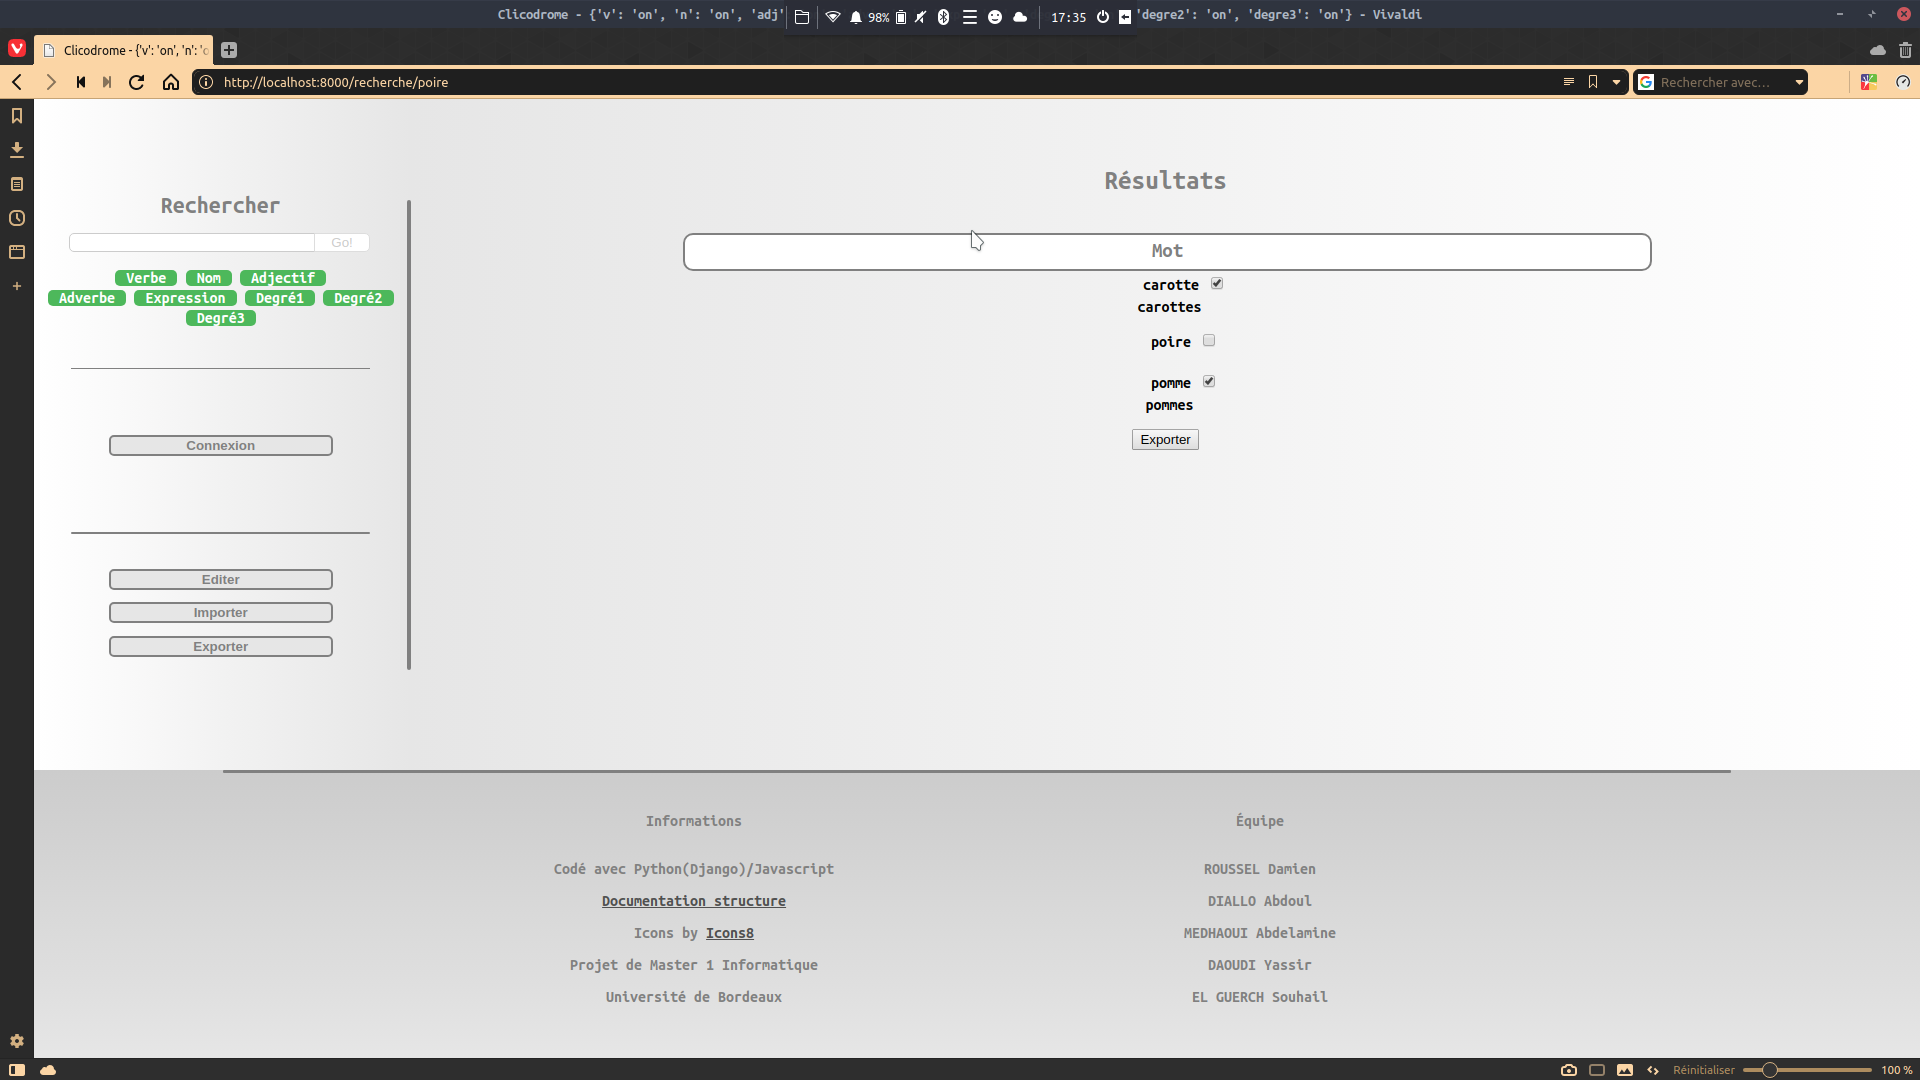
\includegraphics[scale=0.27]{recherche.png}
    \caption{Exemple pour une recherche }
    \end{figure}
    \item \textbf{Affiner une recherche:}\\
    Après une recherche, l'utilisateur peut cliquer sur le résultat pour obtenir plus d'information sur le mot. Il peut donc obtenir différents types d'informations sur le mot (lemme,categories, genre, nombre,...). Selon sa catégorie on peut avoir des expressions qui l'utilisent , ou par exemple quand il s'agit d'un verbe sa conjugaison à différents temps, différents modes et à différentes personnes en utilisant les tables de transformations de ce dernier, enregistrées au préalable.
    \item \textbf{Ajouter un mot:}\\
    Pour ajouter un mot au lexique il faut être connecté et en avoir le droit(être donc contributeur ou administrateur). Pour garantir la cohérence et l'intégrité des données chaque mot a un identifiant unique, donc un mot ne peut être enregistré qu'une seule fois. Un formulaire permet de renseigner le mot, ses différentes informations et la ou les les table(s) de transformations qui lui seront appliquée(s).
    \begin{figure}[H] 
    \centering
    \includegraphics[scale=0.28]{ajout mot.png}
    \caption{Formulaire pour ajouter un mot }
    \end{figure}
    \item \textbf{Modifier un mot:}\\
    la gestion de l'attribution des rôles a été mise en place pour éviter au maximum les erreurs. Seuls des utilisateurs jugés aptes et disposant des connaissances nécessaires en linguistique auront le droit d'être contributeur mais malgré cela il faut reconnaître qu'on est jamais à l'abri d'une faute de frappe ou d'une erreur d'inattention. pour remédier à ça il est possible de modifier un mot via l'interface d'administration.
    \item \textbf{Supprimer un mot:}\\
    Cette fonction peut aussi être utile pour faire l'opération précédente en deux temps c'est à dire supprimer un mot erroné et ajouter le bon comme un nouveau mot. Les langues écrites bien que très stables ne sont pas immuables donc certains mot apparaissent et d'autres mots cessent simplement d'exister donc il est important d'avoir la possibilité de supprimer un mot. Les administrateurs et les contributeurs peuvent supprimer un mot en utilisant l'interface d'administration.
\end{itemize}{}

\subsubsection{Gestion des utilisateurs}
Sur notre application chaque utilisateur inscrit a les droits d'accès, de modification et de suppression de son compte.
\begin{figure}[H] 
    \centering
    \includegraphics[scale=0.27]{edition compte.png}
    \caption{Gestion personnel d'un compte }
\end{figure}
Avec notre framework, pour limiter au maximum les erreurs lors d'ajout d'éléments dans le \textbf{lexique}, nous avons mis en place une interface de gestion avec  \textbf{les rôles suivants}:
\begin{itemize}
\item \textbf{Utilisateur}: un utilisateur simple peut \textbf{s'inscrire, valider, supprimer} son compte, il peut  aussi \textbf{consulter} et \textbf{extraire} le lexique.
\item \textbf{Contributeur}: un contributeur dispose en plus des droits d'un utilisateur simple, la possibilité à souhait de \textbf{manipuler le contenu du lexique} (ajouter,modifier, supprimer un mot du lexique).
\item \textbf{Administrateur}: Un Administrateur joue le rôle de modérateur, en plus des droits d'un contributueur, ce dernier  \textbf{gère les droits} des autres utilisateurs ( il peut donc faire passer un utilisateur simple en contributeur, débouter un contributeur de ses droits et le rétrograder au rang d'utilisateur simple ou carrément bannir un utilisateur et supprimer son compte ).
\begin{figure}[H]
    \centering
    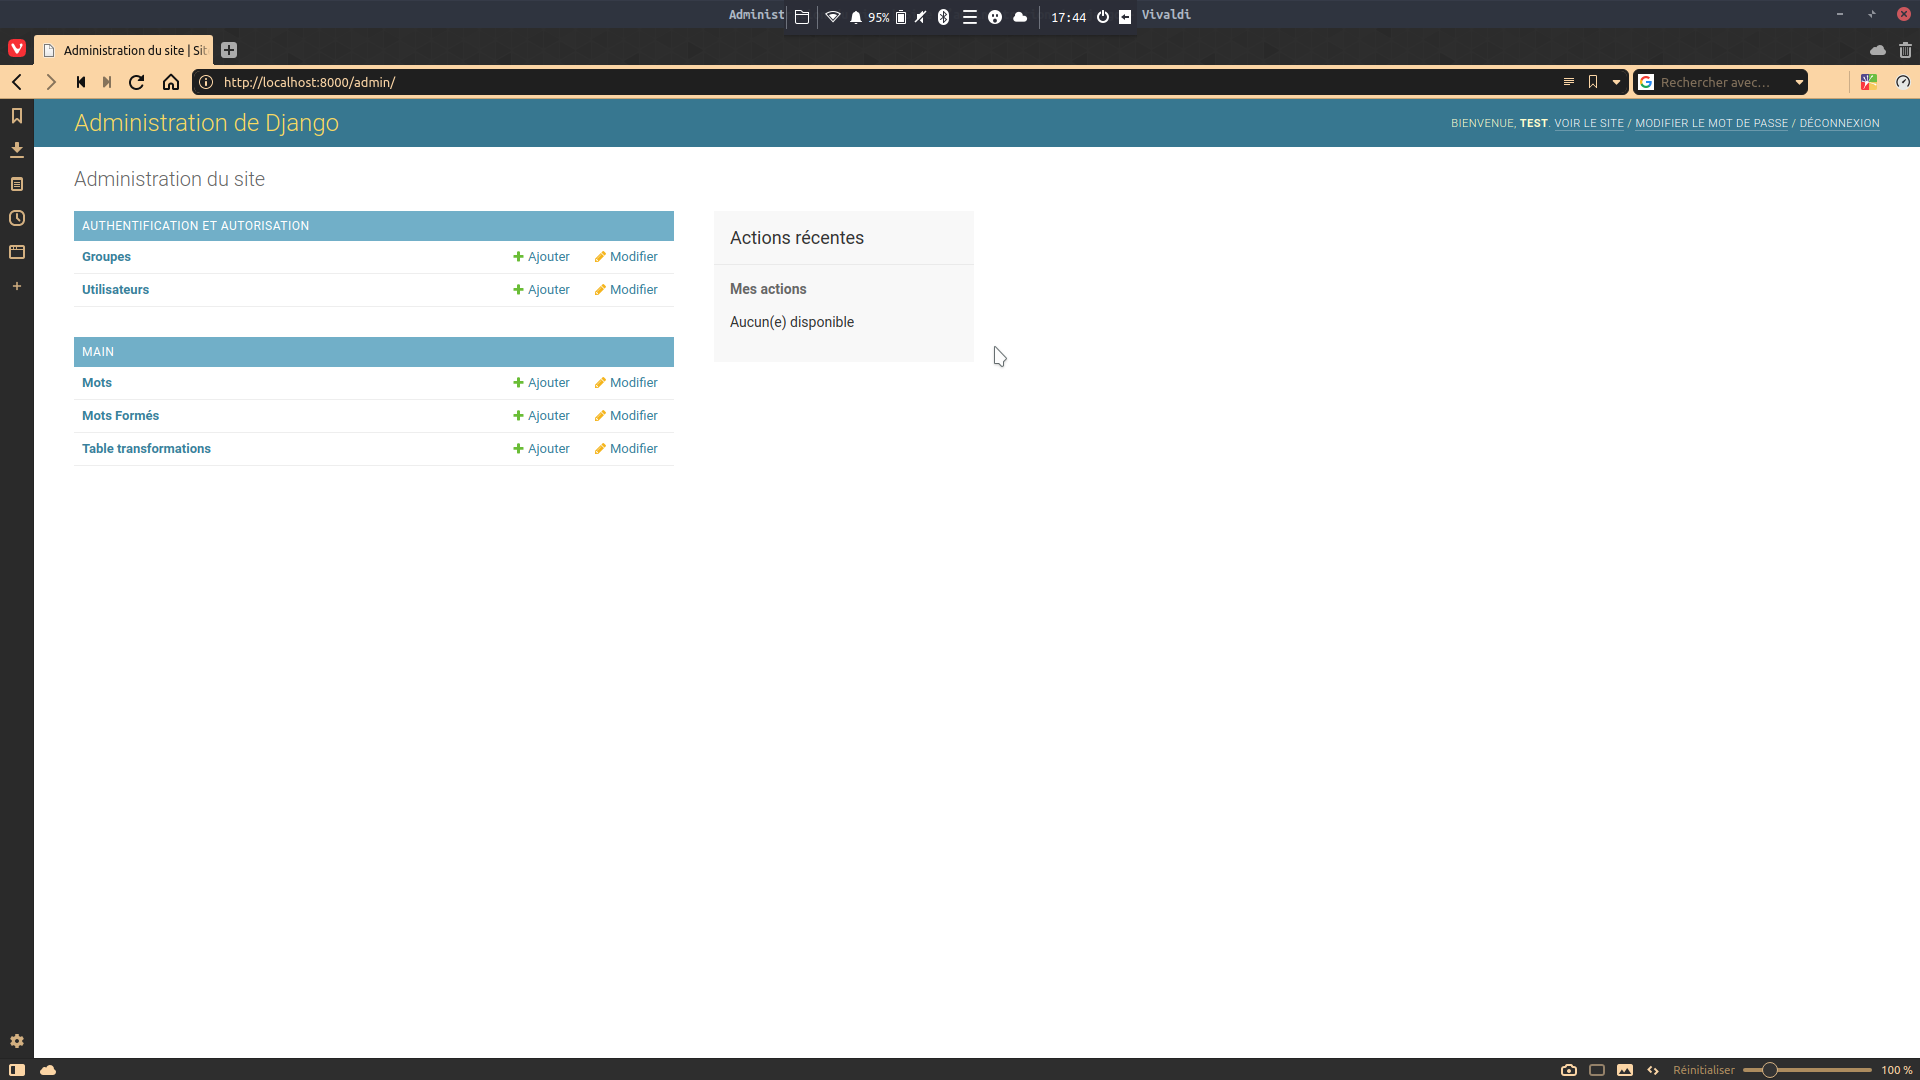
\includegraphics[scale=0.27]{admin.png}
    \caption{Interface d'administration }
\end{figure}
\end{itemize}
Cette façon de gérer les rôles reste simple mais efficace et permet une gestion incontournable des autorisations.

\begin{figure}[H] 
    \centering
    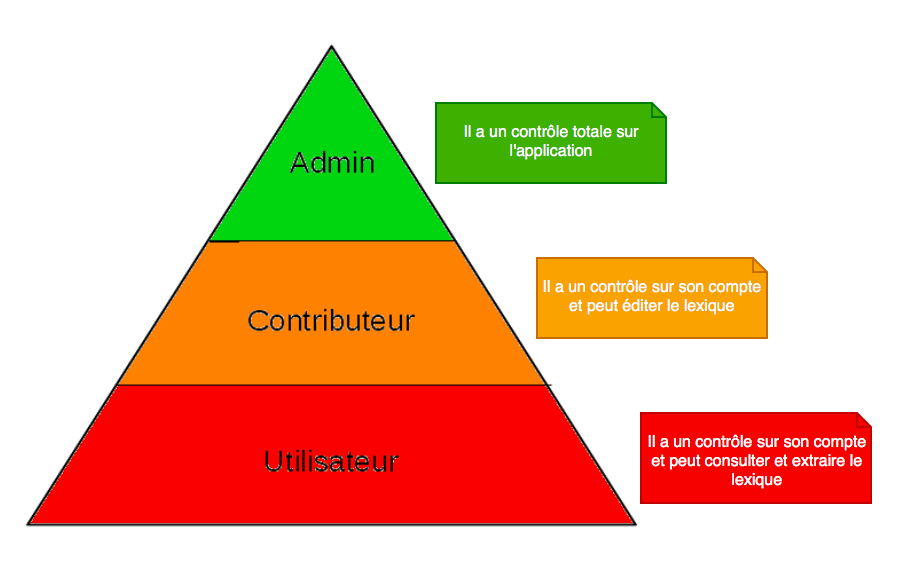
\includegraphics[scale=0.5]{role.png}
    \caption{Gestion des rôles des utilisateurs }
\end{figure}
\newpage

\subsubsection{Les formes fléchies et les catégories de mots}

\begin{itemize}
    \item \textbf{Catégories de mots} \\
        Dans toutes les langues, les mots ont des catégories auxquelles ils appartiennent, il est donc intéressant de pouvoir stocker celles-ci pour pouvoir avoir des informations sur les résultats de la recherche par exemple. Mais aussi pour pouvoir filtrer la recherche en fonction de ces catégories, nous avons donc un système de filtre par catégorie, et par sens.
\item \textbf{Transducteurs} \\
        Un transducteur est une opération qui va appliquer une transformation à un mot, afin de le transformer en une de ses formes possibles, par exemple générer les temps d'un verbe, ou encore masculin/féminin ou bien singulier/pluriel. Cette opération est donc technique puisqu'elle va non seulement transformer un mot en une de ses formes, mais aussi elle doit permettre de rajouter les informations appliquées par cette transformation, pour cela le transducteur fait appel à l'unification.
\begin{figure}[H]
    \centerline{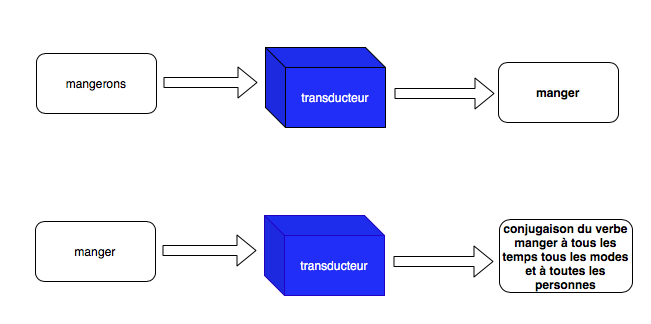
\includegraphics[scale=0.7]{transducteur.png}}
    \caption{Base de données}
\end{figure}

\item \textbf{Unification} \\
        L'unification est une opération qui consiste à tenter de fusionner des informations ensemble, pour cela, il faut vérifier la compatibilité de ces informations entre elles, si jamais des informations sont incompatibles (par exemple singulier et pluriel) dans ce cas l'unification échoue. Si l'opération fonctionne, alors cela signifie que l'on a des informations plus complète sur un mot. Cette opération permet donc de savoir si des mots sont à retourner pour la recherche, ou encore dans un transducteur pour rajouter des informations au mot formé. Pour cela nous avons deux fonctions, une qui va tester si deux mots sont unifiables, et une qui va faire cette tentative de fusion de deux informations. 
\begin{figure}[H]
    \centerline{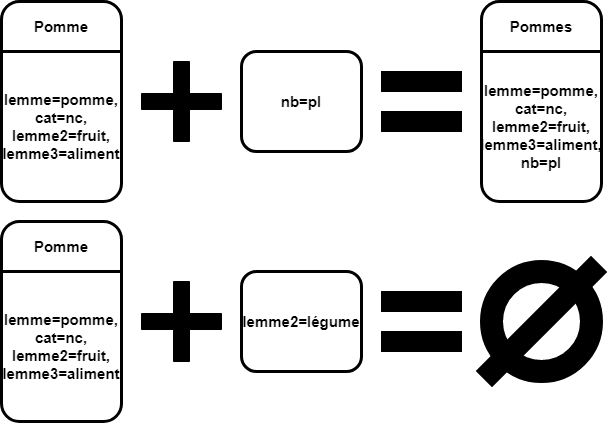
\includegraphics[scale=0.7]{unification.png}}
    \caption{Fonctionnement unification}
\end{figure}
        
\end{itemize}
\subsection{Analyse des besoins non fonctionnels}
\subsubsection{Sécurité}
Le choix d'utiliser un framework n'a pas été anodin dans la construction et la réalisation du projet. En effet, la base de données est une partie importante de l'application web. De ce fait, il a fallu réfléchir aux technologies à mettre en oeuvre pour pouvoir la protéger. \\Comme pour lutter contre une menace de type  \textbf{"Cross site scripting"}, qui est une attaque XSS permettant d'injecter des scripts clients dans les navigateurs des utilisateurs. Des \textbf{scripts malveillants} sont alors stockés dans la base de données d'où ils seront affichés dans le but de pousser les utilisateurs à cliquer sur un lien qui va provoquer l'exécution du JavaScript de l'attaque dans le navigateur des utilisateurs. Afin de pallier à ce genre de menace , le framework  \textbf{Django} permet de nous protéger de la majorités des attaques XSS.\\
La base de données peut être aussi mise en péril par une   \textbf{injection SQL} qui est une menace d'un utilisateur malveillant, capable d'exécuter du code SQL arbitraire dans la base de données. Cette méthode peut mener à des modifications des données. Pour éviter ce genre d'attaque, les jeux de requête du framework Django sont prémunies contre les \textbf{injections SQL} , en effet le code SQL d'une requête est défini séparément de ses paramètres.

\subsubsection{Format de fichier}
\textbf{L'import} et \textbf{l'export} du lexique étant un des \textbf{besoins fonctionnels}, soulève le problème du \textbf{format de fichier} à prendre en charge. A cette question, nous avons décider  dans un premier temps de partir sur un simple \textbf{fichier texte} dont les \textbf{données seront rangées} telle qu'elles sont stockées dans la base de données. Cette version devait être améliorée pour fournir un format xml ou mlex qui faciliterait l'exploitation du lexique par un tiers. 
\subsubsection{Performance}
L'intérêt du site est de pouvoir rechercher du lexique parmi une \textbf{base conséquente de mots} (dans l'idéal tous les mots d'une même langue), ce qui amène le problème de la \textbf{performance} de la fonction de recherche qui est un facteur principal dans l'utilisation du site. En effet une \textbf{mauvaise performance} à ce niveau et le site ne sera que \textbf{très peu utilisé}. De plus le deuxième point problématique est de \textbf{multiples import/export} en même temps sur le serveur, ce qui selon la taille de la base de données peut être très \textbf{gourmand en ressources}. Ces éléments sont donc à prendre en compte afin que l'utilisation du site soit plus agréable.

\subsubsection{Ergonomie}
En ayant une liberté totale à ce niveau, nous avons décidé d'utiliser une \textbf{interface simple et épurée} car l'utilisation principale du site est la \textbf{recherche}, il fallait donc mettre l'accent sur cette fonction qui est \textbf{à tout moment accessible} sur le site. De même nous avons fait en sorte que \textbf{l'accès à un compte} soit \textbf{simple et rapide}, pour permettre d'éditer la base de données si besoin. Enfin la possibilité d'import et d'export du lexique est  aussi accessible à tout moment.
Nous sommes partis sur une version plus élégante et organisée grâce à l'utilisation de boostrap avec Django, cette version était incomplète suite aux circonstances actuelles, mais voici une petite vue sur la page d'accueil :
\\

\centerline{
\includegraphics[scale=0.4]{1.png}}
    
\centerline{
\includegraphics[scale=0.4]{2.png}}
    
\centerline{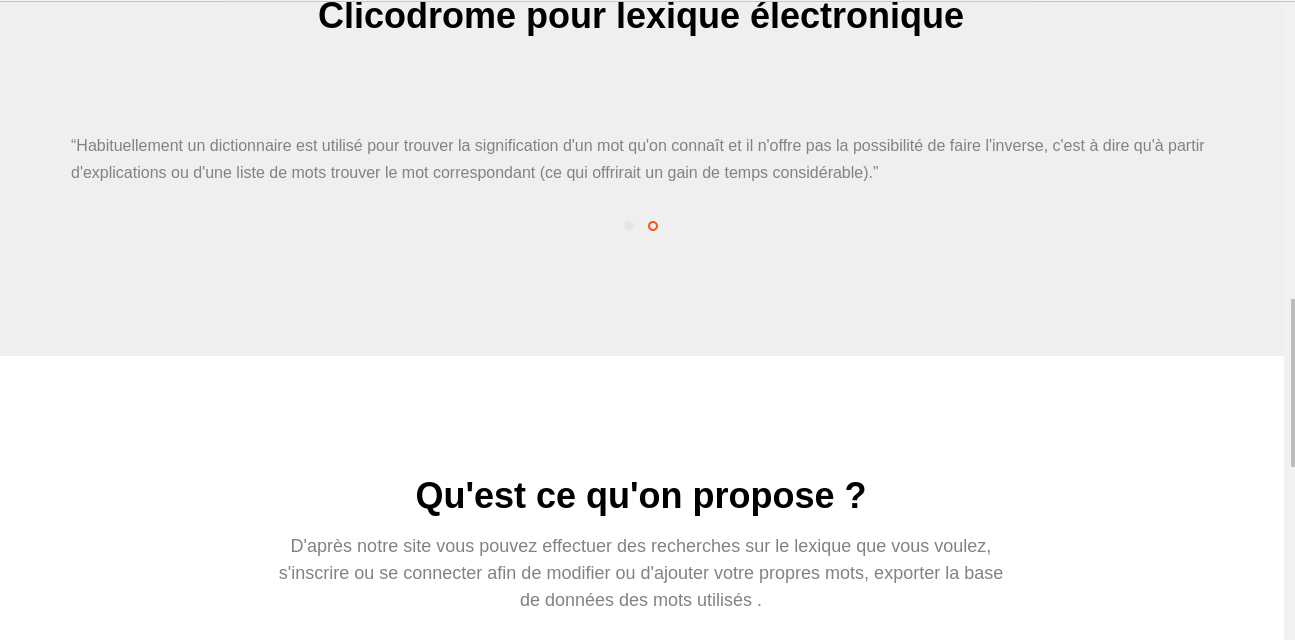
\includegraphics[scale=0.4]{3.png}}

\newpage
    
\section{Architecture et implémentation}
\subsection{La base de données}

Après avoir discuté avec notre client, nous avons constaté que le choix de la forme de la base de données est libre.

Nous avions le choix entre deux formats, La base de données relationnelles : SQL et la non relationnelles NoSQL, et d'après nos recherches, La base de données SQL est la plus convenable pour la conception du projet, vu son coté stable d'utilisation.

Afin de stocker des mots dans cette base de données ,il suffit de choisir un format de stockage qui se base sur une chaîne de caractère bien définie qui va être parsé à la fin dans le but d'extraire les informations sur le mots.
SQL permet aussi l’atomicité ainsi que l’intégrité des données, car avec un seul serveur on peut réaliser de nombreuses requêtes.
Et finalement,les bases de données SQL conviennent parfaitement à l’environnement exigeant des requêtes complexes, qui pourront être exploiter
dans les filtres de recherche ou les algorithmes utilisés.
La base de données contient les tables suivantes :
\begin{figure}[H]
    \centerline{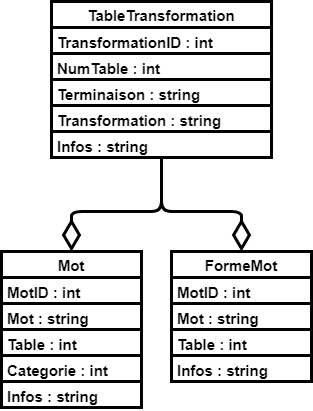
\includegraphics[scale=0.65]{bdd.png}}
    \caption{Base de données}
\end{figure}
\begin{itemize}
    \item \textbf{Mot:}
    Cette table est utilisée pour enregistrer les \textbf{mots} du lexique. Elle référence en plus des options d'affichage : le mot, sa catégorie, ses différentes informations et la table de transformation qui lui est associée.
    \item \textbf{FormeMot:}
    Au lancement de l'application touts les mots formés seront chargés.
    Cette table est utilisée pour enregistrer les \textbf{mots formés} à partir de l'application des opérations de transduction sur les mots de base du lexique. Elle référence en plus des options d'affichage : le nouveau mot,son identifiant (unique cette fois encore), ses différentes informations et la table de transformation qui lui est associée.
    \item \textbf{TableTransformation:}
    Cette table permet d'enregistrer les \textbf{tables de transformation} associés aux différents mot du lexique. Elle contient l'identifiant unique de la table, le numéro de la table(chaque table a un numéro unique il en existerait une centaine pour les verbes par exemple), ainsi que d'autres informations utiles pour les opération de transduction.
    Le champ terminaison représente la partie du mot qui va être remplacer par la transformation.\\
    Cette table sert à implémenter le transducteur.
\end{itemize}
\subsection{L'application Web}
 La figure suivante résume le fonctionnement global du site .
\begin{figure}[H]
    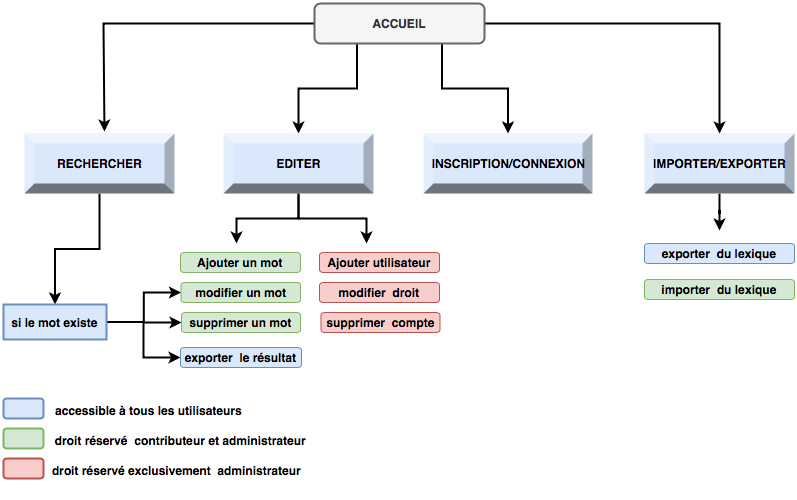
\includegraphics[scale=0.65]{fonctionnement.png}
    \caption{Fonctionnement global de l'application }
\end{figure}
\begin{figure}[H]
    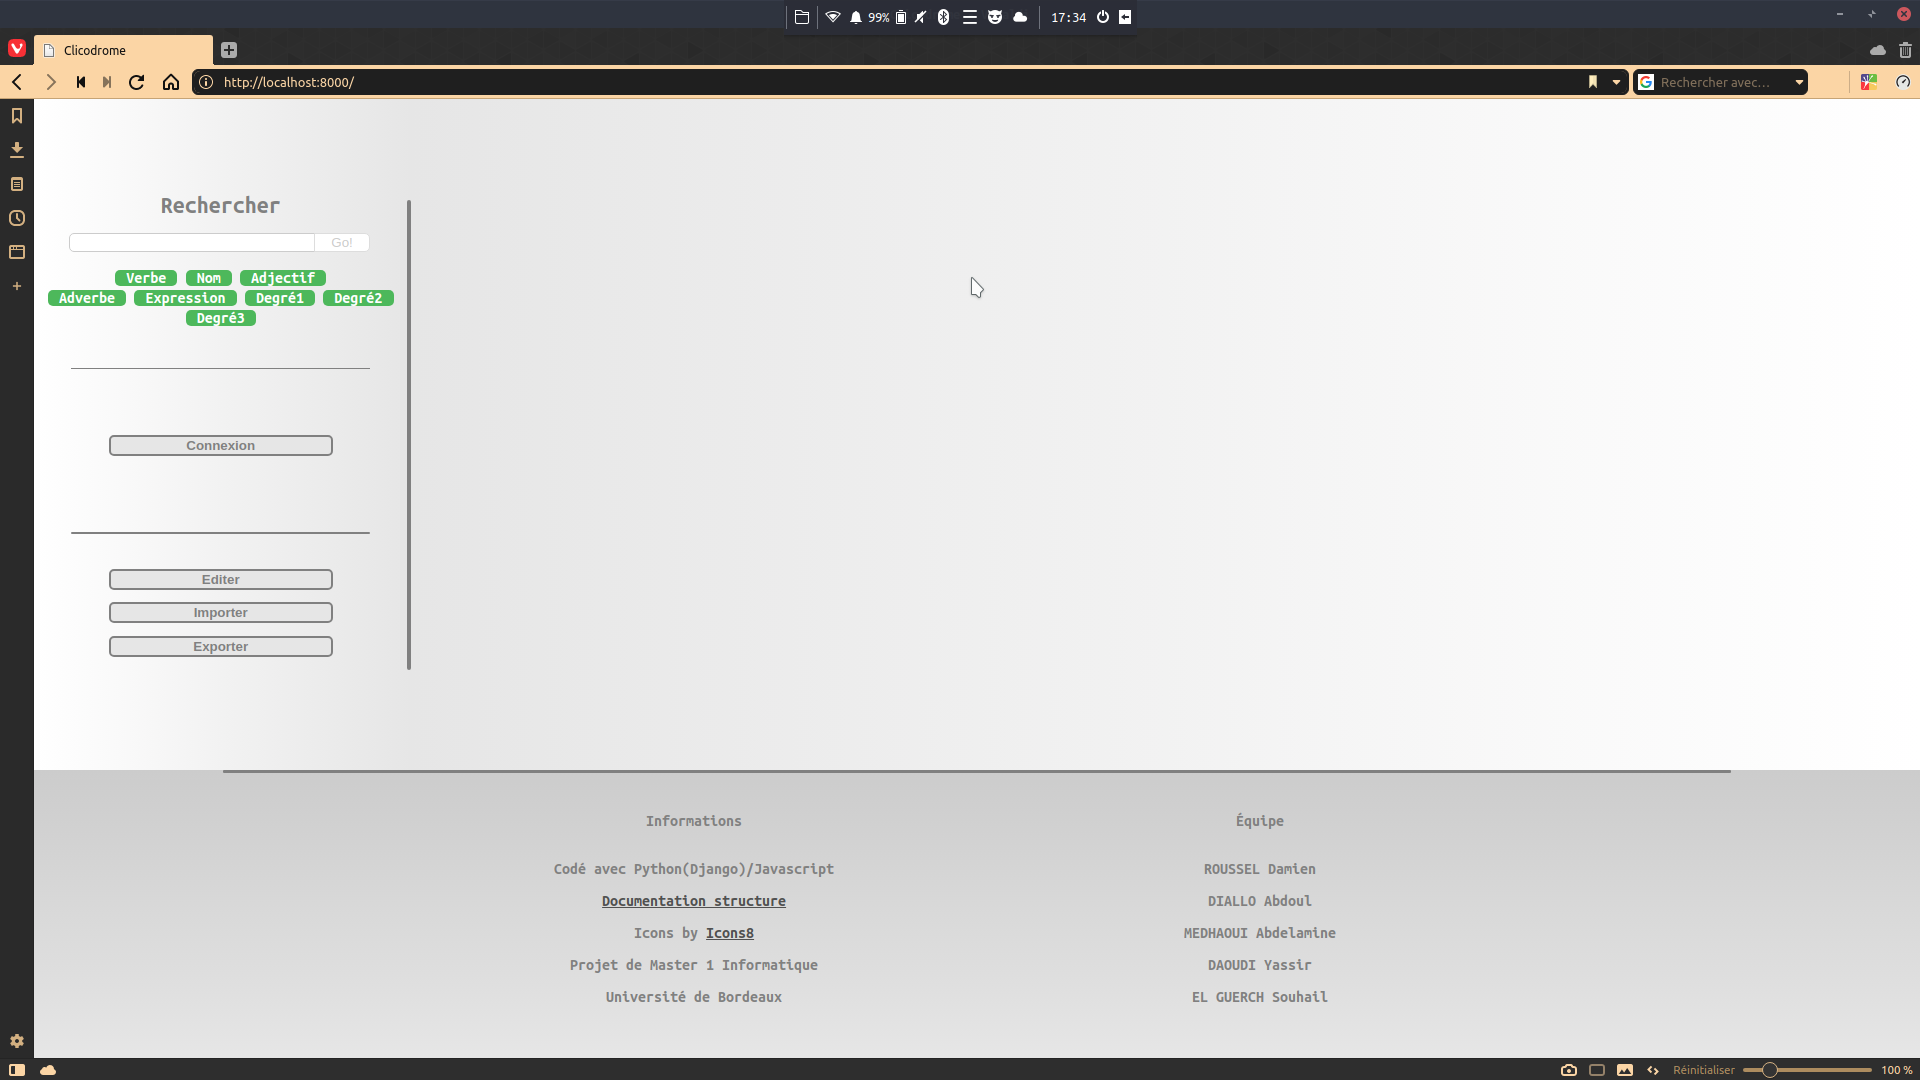
\includegraphics[scale=0.27]{acceuil.png}
    \caption{Page d'accueil du site}
\end{figure}
\begin{figure}[H]
    \includegraphics[scale=0.27]{connexion inscription.png}
    \caption{Se connecter ou S'inscrire }
\end{figure}
\subsection{Outils de développement}
\subsubsection{Le choix du langage de programmation}
Pour le Back-end de notre application, on a décidé à l'unanimité et après une longue concertation de travailler avec le langage python. Cette décision est motivée par la complexité des données à manipuler (lors des opérations de transduction et/ou d'unification). En effet python est un langage à typage dynamique, il dispose de plusieurs fonctionnalités et offre des bibliothèques bien fournies et documentées pour manipuler des données. Nous ajouterons à cela une très grande et active communauté de développeurs et le fait que certains membre du groupe avaient au préalable une expérience dans l'utilisation de ce langage.  
\subsubsection{Le choix du Framework}
Un framework ou traduit littéralement de l'anglais, un cadre de travail est un ensemble d'outils qui facilite le travail des développeurs. Il apporte les bases communes à la majorité des projets de développement. Celles-ci étant souvent identiques (inscription, authentification, connexion,...) d'un projet à l'autre donc un développeur peut simplement les réutiliser et se concentrer sur les particularités de son projet. Pour éviter de réinventer la roue nous avons choisi le Framework Django pour la réalisation de ce projet. Dans l'ensemble la figure suivante illustre le fonctionnement d'une application Django:
 \begin{figure}[H] 
    \centering
    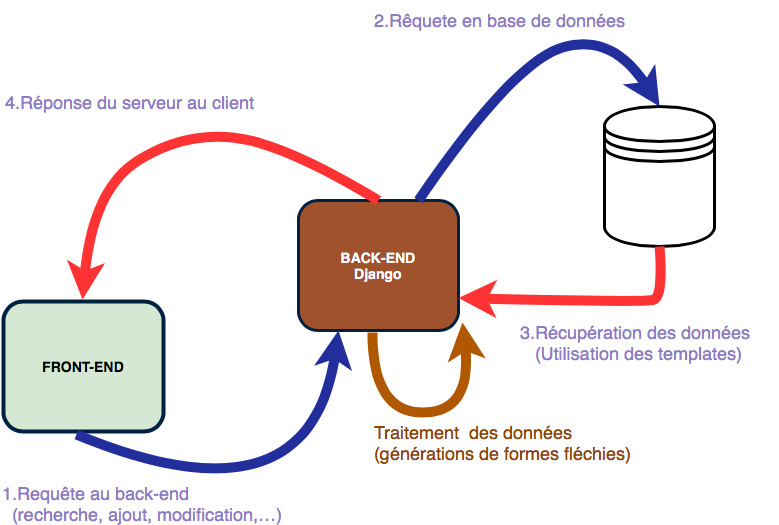
\includegraphics[scale=0.65]{fct.png}
    \caption{ajout de nouvelles fonctionnalités }
    \end{figure}
Ce framework offre plusieurs fonctionnalités dont entre autres:
\begin{itemize}
    \item Un \textbf{ORM} : est un ensemble de classes permettant de manipuler les tables d’une base de données relationnelle comme s’il s’agissait d’objets. c'est donc une couche d’abstraction d’accès à la base de données qui donne l’illusion de ne plus travailler avec des requêtes mais de manipuler des objets.L’avantage de cette couche d’abstraction est qu’on a plus à se soucier du système de gestion base de données utilisé, c’est l’ORM qui a la charge de transformer les requêtes pour les rendre compatibles avec la base de données.L’ORM va s’appuyer sur des modèles. Un modèle représente une table de la base de données.
    \begin{figure}[H] 
    \centering
    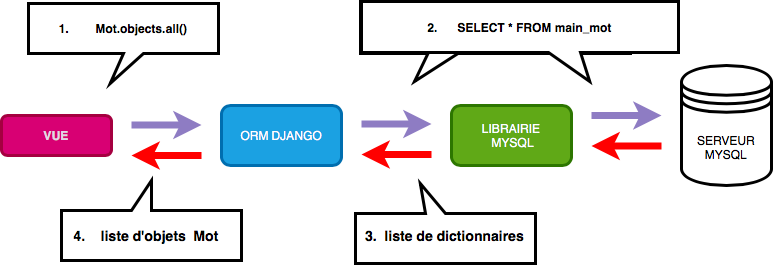
\includegraphics[scale=0.65]{orm.png}
    \caption{Fonctionnement de L'ORM de Django }
    \end{figure}
    \item Un projet Django est composée de plusieurs application structurées de la même manière. Cela facilite la réutilisation des applications existantes et  donc par conséquent l'\textbf{ajout de nouvelles fonctionnalités} à un projet. Actuellement notre client cherche un outil pour faciliter l'usage du \textbf{LeFFF} si dans un futur proche il veut rajouter un forum de discussion ou une rubrique qui traite de divers sujets en linguistique il suffit de créer ces nouvelles applications ou de les trouver et les intégrer au projet originel en adaptant les URL du sites. 
    \begin{figure}[H] 
    \centering
    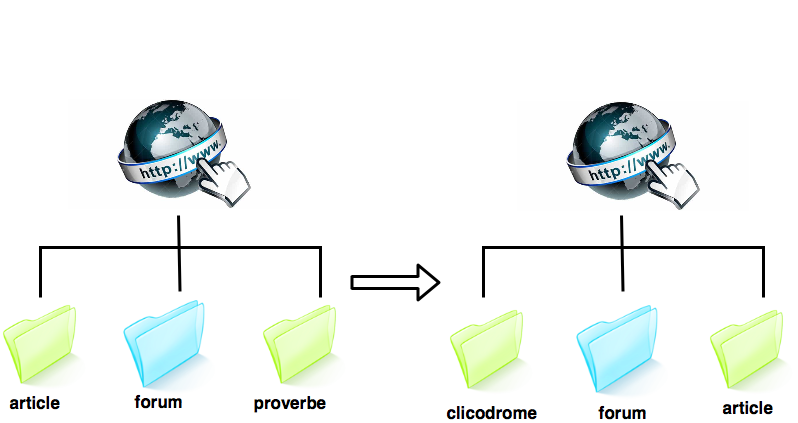
\includegraphics[scale=0.65]{portabilite.png}
    \caption{ajout de nouvelles fonctionnalités }
    \end{figure}
\end{itemize}
\subsubsection{La base de données}
Sur recommandation de notre client nous avons choisi MySQL comme Système de Gestion de Base de Données(SGBD). Mais avec l'utilisation de django il est facile de changer de SGBD car grace à son ORM nous ne nous occupons pas de réecrire les requêtes SQL. 

\section{analyse du fonctionnement et tests}
Le framework offre un fichier  \verb+test.py+  pour tester notre application. Nous avions fait le choix de tester au fur et à mesure qu'on écrivait du code et ajoutait de nouvelles fonctionnalités.
\subsection{Tests unitaires}
On a donc tester les différentes fonctions essentielles de l'application:
\begin{itemize}
    \item \textbf{Ajouter un mot} : la structure de la base de données ne permet en aucun cas l'existence de doublons. La complexité de la langue française fait qu'on peut avoir beaucoup de confusions en passant de l'oral à l'écrit. Par exemple on peut avoir : "suis" pour la conjugaison du verbe être à la première personne du singulier et  au présent de l'indicatif qui est identique à "suis" qui est la conjugaison du verbe suivre à la première personne du singulier au présent de l'indicatif. Mais il n'y aura pas de problème pour l'enregistrement car bien qu'ils s'écrivent de manière identique ce n'est pas le même verbe.
    \item \textbf{Modifier un mot }: la modification d'un mot comme son nom l'indique ne crée pas un nouveau mot. cette opération garde l'ancien et y apporte la mise à jour nécessaire. Une opération de recherche ne trouvera plus l'ancienne version elle n'existera plus.
    \item \textbf{Supprimer un mot }: la suppression d'un mot entraîne sa disparition définitive de la base de données. Il est impossible de le retrouver avec la fonction de recherche.
    \item \textbf{Rechercher un mot} : la fonction de recherche est développée pour fonctionner avec des filtres pour affiner la recherche. Elle fournit donc des résultats incluant des sens à différents degrés d'application. Chercher le mot pommes en filtrant que c'est un fruit pourra donc nous sortir les autres mots étiquetés comme étant des fruits.
\end{itemize}{}
\subsection{Test de performances}
Les tests de performance concernent essentiellement les fonctions d'import et d'export de lexique. Pour obténir des données à importer nous avons utilisé l'outil \verb+scapy+ de python qui permet de sniffer des pages sur internet (des dictionnaires essentiellement) en d'en extraire les informations qui nous intéressent via les balises html de celles-ci. Une fois ces données à disposition on a effectuer plusieurs tests avec des temps de réalisation variables d'une machine à l'autre  mais tout de même satisfaisants.  
\\
Les manques de performance aussi peuvent se manifester lors d'un test de connexion de plusieurs clients pour un serveur. En effet, grâce à l'architecture Model View Template (MVT) de Django  qui permet de parcourir les fichiers de manière simple et efficace et aux fonctions qui ne sont pas gourmandes en mémoire, la gestion simultanée de plusieurs connexions n'entraînera pas de ralentissement du site.  

\section{Conclusion}

{La réalisation de ce projet nous a permis :
\begin{itemize}
    \item d'acquérir les concepts principaux du génie logiciel et de les mettre en application : besoins fonctionnels et non fonctionnels, conception et spécification, tests, architecture et modularité, outils d'aide au développement, travail en équipe.
    \item de renforcer nos connaissances en programmation : paradigmes de programmation, langages de programmation, gestion des erreurs.
    \item d'appliquer une pratique scientifique rigoureuse en développement logiciel : recherche et analyse de l'existant, bibliographie, assimilation de nouveaux concepts, justification des choix, analyses et critiques du travail réalisé, rédaction de documents(rapport hebdomadaire, cahiers des besoins et mémoire).
    \item de découvrir le domaine de la linguistique formelle et du traitement automatique des langues. 
    \end{itemize}{}\par}
{Malgré des conditions de fin de projet difficiles liées à la fermeture de l'université, nous avons un outil qui traite les besoins essentiels du client avec les possibilités d'améliorations suivantes :
    \begin{itemize}
        \item améliorer la rigueur dans l'encadrement des opérations d'interactions avec le lexique pour qu'il puisse être enrichi par le plus grand nombre d'utilisateurs (pas seulement des linguistes). 
        \item ajouter de nouveaux formats notamment .xml et .mlex pour l'import et l'export de lexique
        \item permettre sous encadrement des administrateurs aux utilisateurs simples n'ayant pas le droit d'édition  de faire des suggestions de modification ou d'ajout de mots dans le lexique 
        \item améliorer la fonction de recherche , les opérations de transduction et d'unification pour obtenir plus de performances.
    \end{itemize}{}\par}
    
    Nous ne saurons terminer ce mémoire sans remercier toutes les personnes qui, de près ou de loin ont contribué à la réussite de ce projet. Nous pensons au professeur chargé du cours \textbf{Monsieur PHILIP NARBEL} pour ses aiguillages, au client \textbf{Monsieur LIONEL CLEMENT} pour sa disponibilité et son implication tout au long du processus et au chargé de TD \textbf{Monsier SIMON ARCHIPOFF} pour son encadrement et ses divers conseils.
\newpage
\section{Bibliographie}
\nocite{*}
\printbibliography

\end{document}
